\section{Mapserver}
MapServer adalah sebuah aplikasi freeware dan open source yang dapat menampilkan data spasial (peta) pada web. Aplikasi ini dikembangkan pertama kali oleh Universitas Minesotta, Amerika Serikat dalam projek ForNet yang merupakan sebuah projek untuk manajemen sumber daya alam yang disponsori NASA. kemudian dikembangkan projek TerraSIP sebagai manajemen data lahan. Karena sifatnya terbuka atau open source, pengembangan MapServer dilakukan oleh banyak negara.

Map Server bekerja beriringan dengan aplikasi web server. Web Server menerima request peta melalui MapServer, lalu MapServer mengenerate request terhadap peta lalu mengirimkannya ke web server seperti gambar dibawah ini.
\begin{figure}[ht]
	    \centerline{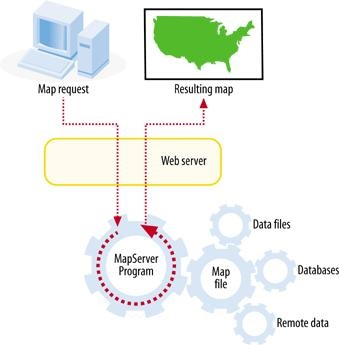
\includegraphics[width=0.50\textwidth]{figures/gambar5.JPG}}
	    \caption{Diagram operasi standar pada MapServer}
		\label{gambar5}
		\end{figure}
Fungsi utama dari MapServer yaitu untuk melakukan pembacaan data dari berbagai sumber dan menempatkannya kedalam layer-layer secara bersamaan yang kemudian menjadi file graphic.

Mapserver menghasilkan keluaran berupa file graphic berdasarkan masukan yang diberikan oleh user. Komponen kuncinya adalah MapServer executable yang terdiri dari CGI program, file peta, sumber data dan output gambar. Seperti pada gambar dibawah ini semua komponen bekerja bersama-sama, setelah user melakukan request/perminataan maka CGI akan mengakses file peta, menggambarkan informasi yang didapat dari sumber data dan kembali menampilkannya pada peta.

\subsection{Pengertian MS4W}
MapServer for Windows (MS4W) adalah suatu packet software untuk mempermudah pengguna dalam menginstalasi MapServer pada platform OS Microsoft Windows. Tujuannya adalah untuk mempermudah semua user, terhindar dari segala bagian kecil yang rumit dalam mempersiapkan lingkungan kerja yang dibutuhkan oleh MapServer pada lingkungan Microsoft Windows. Software ini juga merupakan suatu cara yang bagus dalam memaketkan kemudian mendistribusikan aplikasi-aplikasi MapServer kepada pihak manapun.

\subsubsection{Komponen MS4W}
Paket dasar MS4W terdiri dari beberapa komponen sebagai berikut:
\item Webserver Apache
\item PHP
\item MapServer CGI
\item PHP/Mapscript
\item Program utiliti (pustaka) GDAL & OGR
\item Program utiliti MapServer (shp2img, legend, scalebar, sortshp, sym2img, shptree, dan tile4ms)
\item Ekstensi OGR/PHP
\item OWTChart

\subsection{Cara Instalasi Mapserver}
\begin{enumerate}
\item
Download Mapserver atau disingkat MS4W di http://mapserver.org/download.html
\begin{figure}[ht]
	    \centerline{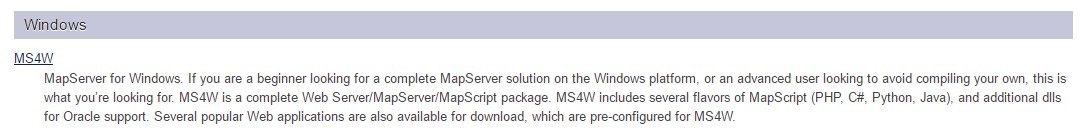
\includegraphics[width=0.50\textwidth]{figures/gambar1.JPG}}
	    \caption{Download MS4W}
		\label{gambar1}
		\end{figure}
\item
Setelah di download jalankan setupnya, disini saya menggunakan port 2000 karena port default 80 sudah dipakai oleh xampp
\begin{figure}[ht]
	    \centerline{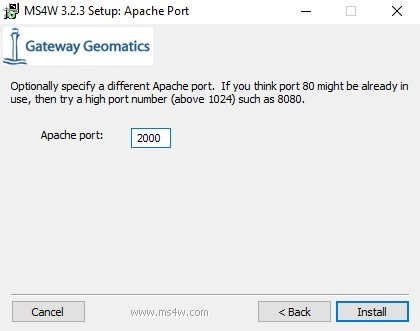
\includegraphics[width=0.50\textwidth]{figures/gambar2.JPG}}
	    \caption{Port 2000}
		\label{gambar2}
		\end{figure}
\item
Lalu tunggu instalasi sampai selesai
\begin{figure}[ht]
	    \centerline{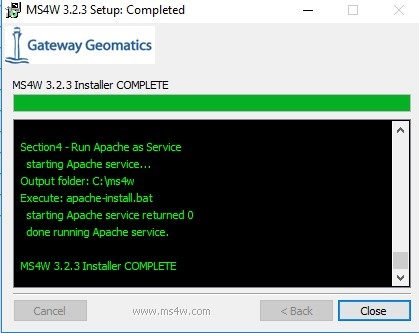
\includegraphics[width=0.50\textwidth]{figures/gambar3.JPG}}
	    \caption{Selesai}
		\label{gambar3}
		\end{figure}
\item
Setelah proses selesai silahkan buka browser favorit anda, kemudian ketikkan http://localhost:2000 di kotak isian URL.
\item
Jika anda melihat tampilan home MAPSERVER atau MS4W proses instalasi anda berhasil.
\begin{figure}[ht]
	    \centerline{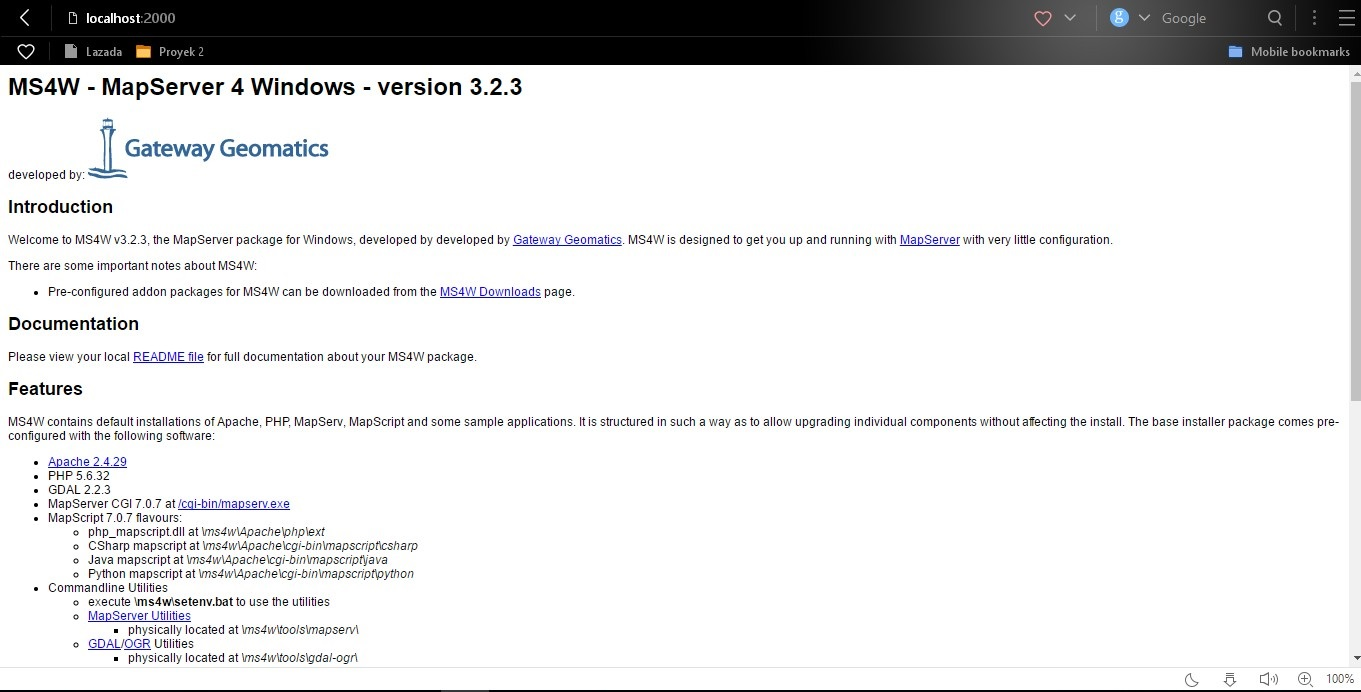
\includegraphics[width=0.50\textwidth]{figures/gambar4.JPG}}
	    \caption{Tampilan MS4W}
		\label{gambar4}
		\end{figure}
\end{enumerate}


\subsection{Arsitektur}
\begin{figure}[ht]
	    \centerline{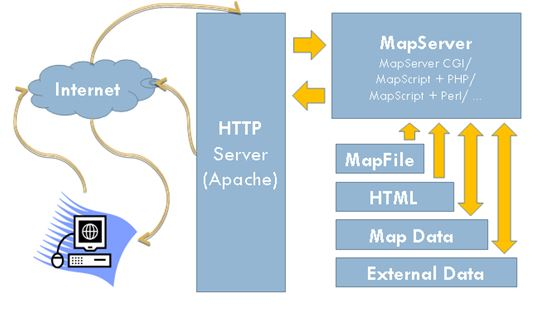
\includegraphics[width=0.50\textwidth]{figures/gambar6.JPG}}
	    \caption{Arsitektur}
		\label{gambar6}
		\end{figure}
Pada sistem aplikasi ini, browser (client) mengirimkan request (melalui jaringan internet/intranet) ke web server dalam bentuk request terkait spasial (lokasi[x,y] click kursor, status [on/off] layer yang akan dimunculkan, dsb).
Kemudian oleh web server, request terkait spasial ini dikirim ke server aplikasi (yang dibangun dengan menggunakan pemograman script yang telah tersedia) dan Mapserver (program CGI). Setelah itu, Mapserver akan membaca mapfile, data peta, dan data eksternal (jika ada dan memang diperlukan).
Setelah itu, gambar akan dikirim ke web server dan akhirnya browser milik client. Arsitektur Mapserver cenderung bercirikan thin-client.

\section{Arsitektur Dasar Aplikasi MapServer}
Map File - file konfigurasi teks terstruktur untuk aplikasi MapServer Anda. Ini mendefinisikan area peta Anda, memberi tahu program MapServer tempat data Anda berada dan di mana menampilkan gambar.
Data Geografis - MapServer dapat memanfaatkan banyak jenis sumber data geografis. Format defaultnya adalah format ESRI Shape.
HTML Pages - antarmuka antara pengguna dan MapServer. Mereka biasanya duduk di root Web. Dalam bentuknya yang paling sederhana, MapServer dapat dipanggil untuk menempatkan gambar peta statis pada halaman HTML. Untuk membuat peta interaktif, gambar ditempatkan dalam bentuk HTML pada halaman.
MapServer CGI - File biner atau executable yang menerima permintaan dan mengembalikan gambar, data, dan lain-lain. Ini ada di direktori cgi-bin atau script dari server web.
Web / HTTP Server - menyajikan halaman HTML saat dilanda browser pengguna.
